\documentclass[12pt,a4paper]{article}
\usepackage[UTF8]{ctex}
\usepackage{amsmath,amssymb}
\usepackage{listings}
\usepackage{xcolor}
\usepackage{hyperref}
\usepackage{geometry}
\usepackage{graphicx}
\geometry{margin=2.5cm}

\lstdefinestyle{python}{
  language=Python,
  basicstyle=\ttfamily\small,
  keywordstyle=\color{blue}\bfseries,
  commentstyle=\color{gray},
  stringstyle=\color{red},
  showstringspaces=false,
  breaklines=true,
  frame=single,
  backgroundcolor=\color{gray!10}
}

\title{Quantum Clustering / 量子聚类}
\author{QuoNic}
\date{}

\begin{document}
\maketitle

\begin{center}
\textbf{ML / 机器学习} | 难度：高级 | 预计时间：20 分钟
\end{center}

\tableofcontents
\newpage

\section{为什么需要？}

量子聚类是经典聚类算法的量子推广，利用量子计算加速聚类。

\subsection{经典局限}
\begin{itemize}
  \item 经典聚类算法（如 K-means）需要 $O(NKd)$ 时间
  \item 对于大规模数据，经典方法效率低
\end{itemize}

\subsection{量子优势}
\begin{itemize}
  \item 量子聚类可以利用量子并行性加速
  \item 可以处理高维数据
  \item 提供量子优势
\end{itemize}

\subsection{实际应用}
\begin{itemize}
  \item 数据分析
  \item 图像处理
  \item 模式识别
\end{itemize}

\section{快速上手}

\begin{lstlisting}[style=python]
from quonic.ml import quantum_clustering

# Quantum clustering
data = [[0, 1], [1, 0], [1, 1], [0, 0]]
result = quantum_clustering(data, n_clusters=2)
print(f"Labels: {result.labels}")
\end{lstlisting}

\textbf{预期输出}：
\begin{verbatim}
Labels: [0, 1, 1, 0]
\end{verbatim}

\section{原理详解}

\subsection{电路图}

\begin{center}
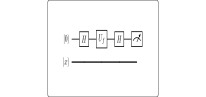
\includegraphics[width=0.6\textwidth]{../../images/quantum_clustering_circuit.svg}
\end{center}

\subsection{数学推导}

量子聚类基于量子距离估计：
\begin{equation}
d(x_i, x_j) = 1 - |\langle\phi(x_i)|\phi(x_j)\rangle|^2
\end{equation}

\textbf{算法步骤}：
\begin{enumerate}
  \item 将数据编码到量子态
  \item 用量子距离估计计算距离矩阵
  \item 用经典聚类算法（如 K-means）聚类
\end{enumerate}

\subsection{几何解释}

量子聚类将数据映射到量子态空间，通过量子距离估计计算距离，然后用经典算法聚类。

\section{代码详解}

\begin{lstlisting}[style=python]
from quonic.ml import quantum_clustering

# quantum_clustering(data, n_clusters, shots)
# data: input data points
# n_clusters: number of clusters
# shots: number of measurements
result = quantum_clustering(data, n_clusters=2, shots=1024)

# result.labels: cluster labels
# result.centroids: cluster centroids
print(f"Labels: {result.labels}")
\end{lstlisting}

\section{进阶用法}

\subsection{场景 1：不同数据}

\begin{lstlisting}[style=python]
# Different datasets
data1 = [[0, 1], [1, 0], [1, 1], [0, 0]]
result1 = quantum_clustering(data1, n_clusters=2)

data2 = [[0, 0, 1], [1, 0, 0], [0, 1, 0], [1, 1, 1]]
result2 = quantum_clustering(data2, n_clusters=2)
\end{lstlisting}

\section{适用场景}

\subsection{数据分析}

量子聚类可以用于大规模数据分析。

\subsection{图像处理}

量子聚类可以用于图像分割和分类。

\section{常见问题}

\subsection{量子聚类的优势是什么？}

量子聚类可以利用量子并行性加速距离计算。

\subsection{量子聚类的局限性是什么？}

需要能够高效编码数据到量子态。

\section{学习路径}

\subsection{前置知识}
\begin{itemize}
  \item 聚类算法
  \item 量子核方法
  \item 量子态编码
\end{itemize}

\subsection{继续学习}
\begin{itemize}
  \item 量子 SVM
  \item 量子神经网络
  \item 量子降维
\end{itemize}

\section{完整示例代码}

\subsection{示例 1：基本量子聚类}

\begin{lstlisting}[style=python]
from quonic.ml import quantum_clustering

data = [[0, 1], [1, 0], [1, 1], [0, 0]]
result = quantum_clustering(data, n_clusters=2)
print(f"Labels: {result.labels}")
\end{lstlisting}


\section{下载}

\begin{itemize}
  \item [quantum_clustering.py](https://github.com/ChrisLee0721/QuoNic/blob/main/examples/quantum_clustering/quantum_clustering.py)
\end{itemize}

\end{document}
